%!TEX root = ../dissertation.tex
\begin{savequote}[75mm]
HAMLET: Do you see yonder cloud that’s almost in shape of a camel?\\
POLONIUS: By th' mass, and ’tis like a camel indeed.\\
HAMLET: Methinks it is like a weasel.\\
POLONIUS: It is backed like a weasel.\\
HAMLET: Or like a whale.\\
POLONIUS: Very like a whale.\\
\qauthor{Shakespeare -- Hamlet, Act 3, Scene 2}
\end{savequote}


\chapter{Characterizing conventions: the dynamics of structure and content}
\graphicspath{{./figures/tangrams/}}

Talking with new partners about new referents poses a challenging coordination problem for social agents. 
The computational approach developed in Chapters 2 and 3 explains key qualitative features of how speakers may solve this problem, and models derived from this approach function reasonably well in repeated reference games with humans. 
However, further model development depends critically upon a finer-grained characterization of the \emph{quantitative} signatures of semantic adaptation found in human communication. 
%That is, distinguishing among different models requires  measurements 
Certain fundamental descriptive questions remain unanswered, and important theoretical constructs remain poorly operationalized. 

% in this literature. %on repeated reference games has extensively established a number of important qualitative properties of convention formation through careful experimental manipulations (see Chapter 1), but 
For example, it has been widely observed that utterances reduce in length as common ground is accumulated.
But a precise characterization \emph{what} gets reduced, and \emph{how}, has remained elusive.
How systematic is the structure of reduction over time?
Which sets of words are dropped together and in what sequence?
What determines whether a particular word is dropped or preserved? 
Similarly, while theoretical definitions of constructs like arbitrariness or stability have loomed over the theoretical analysis of conventions \cite{Lewis69_Convention}, it has been unclear how exactly to measure the extent to which these properties hold in a particular task and how they may evolve over the course of interaction. 
Without addressing these gaps in measurement, it is difficult to set criteria to distinguish among different models.

%While a lifetime of learning the conventions of our language community provides a crucial backbone for understanding each other \cite{Lewis69_Convention}, we frequently find ourselves in situations where our existing lexicon falls short.
%For one, no two speakers share exactly the same lexicon \cite{Davidson86_DerangementOfEpitaphs, Clark98_CommunalLexicons}. 
%Lingo, proper nouns, nicknames, slang, inside jokes, metaphors, and other creative uses of neologism all operate in a regime of uncertainty where the same word or phrase may \emph{a priori} mean something different (or nothing at all) to different partners in different contexts. (cite, cite).
%At the same time, because we live in a changing environment, we constantly experience novel entities, events, thoughts, and feelings we want to talk about---complex referents for which we have no pre-existing conventions and real uncertainty about whether a novel compositional expression will mean to our partner exactly what we intend it to mean.
%What do we do when our lexicon isn't sufficient --- when we have to talk about something we've never had to talk about before with a partner we've never met?

In this chapter, we examine these questions in a large corpus of referring expressions from a new web-based replication of the classic Tangrams task \cite{ClarkWilkesGibbs86_ReferringCollaborative}.
The computational techniques necessary to analyze such rich natural language data were limited at the time of prior work, but have become newly tractable given developments in natural language processing (NLP). 
Our analyses divide into two broad categories roughly corresponding the dynamics of \emph{content} and \emph{structure} of referring expressions across interaction.
To examine content, we extracted word embeddings (e.g. GloVe vectors) for each message to calculate the similarity of messages within and across pairs. 
We found that while different pairs coordinate on a wide range of idiosyncratic solutions to the problem of reference, they do so in an increasingly stable and path-dependent manner. 
Further, words that are more discriminative in the initial context (i.e. that were used for one target more than others) are more likely to persist through the final round. 
To examine structure, we extracted parts of speech and syntax trees from the text to understand what was reducing and how.
We found that pairs systematically drop entire modifying phrases at each repetition, leaving only open-class parts of speech (e.g. an adjective and noun) by the final round. 
These findings provide higher resolution into the quantitative dynamics of convention formation and support the modeling framework introduced in earlier chapters. 
Based on usage, new meanings are systematically grounded with a partner to support more efficient communication.

\section{Methods: Repeated reference experiment}

\begin{figure}
\centering
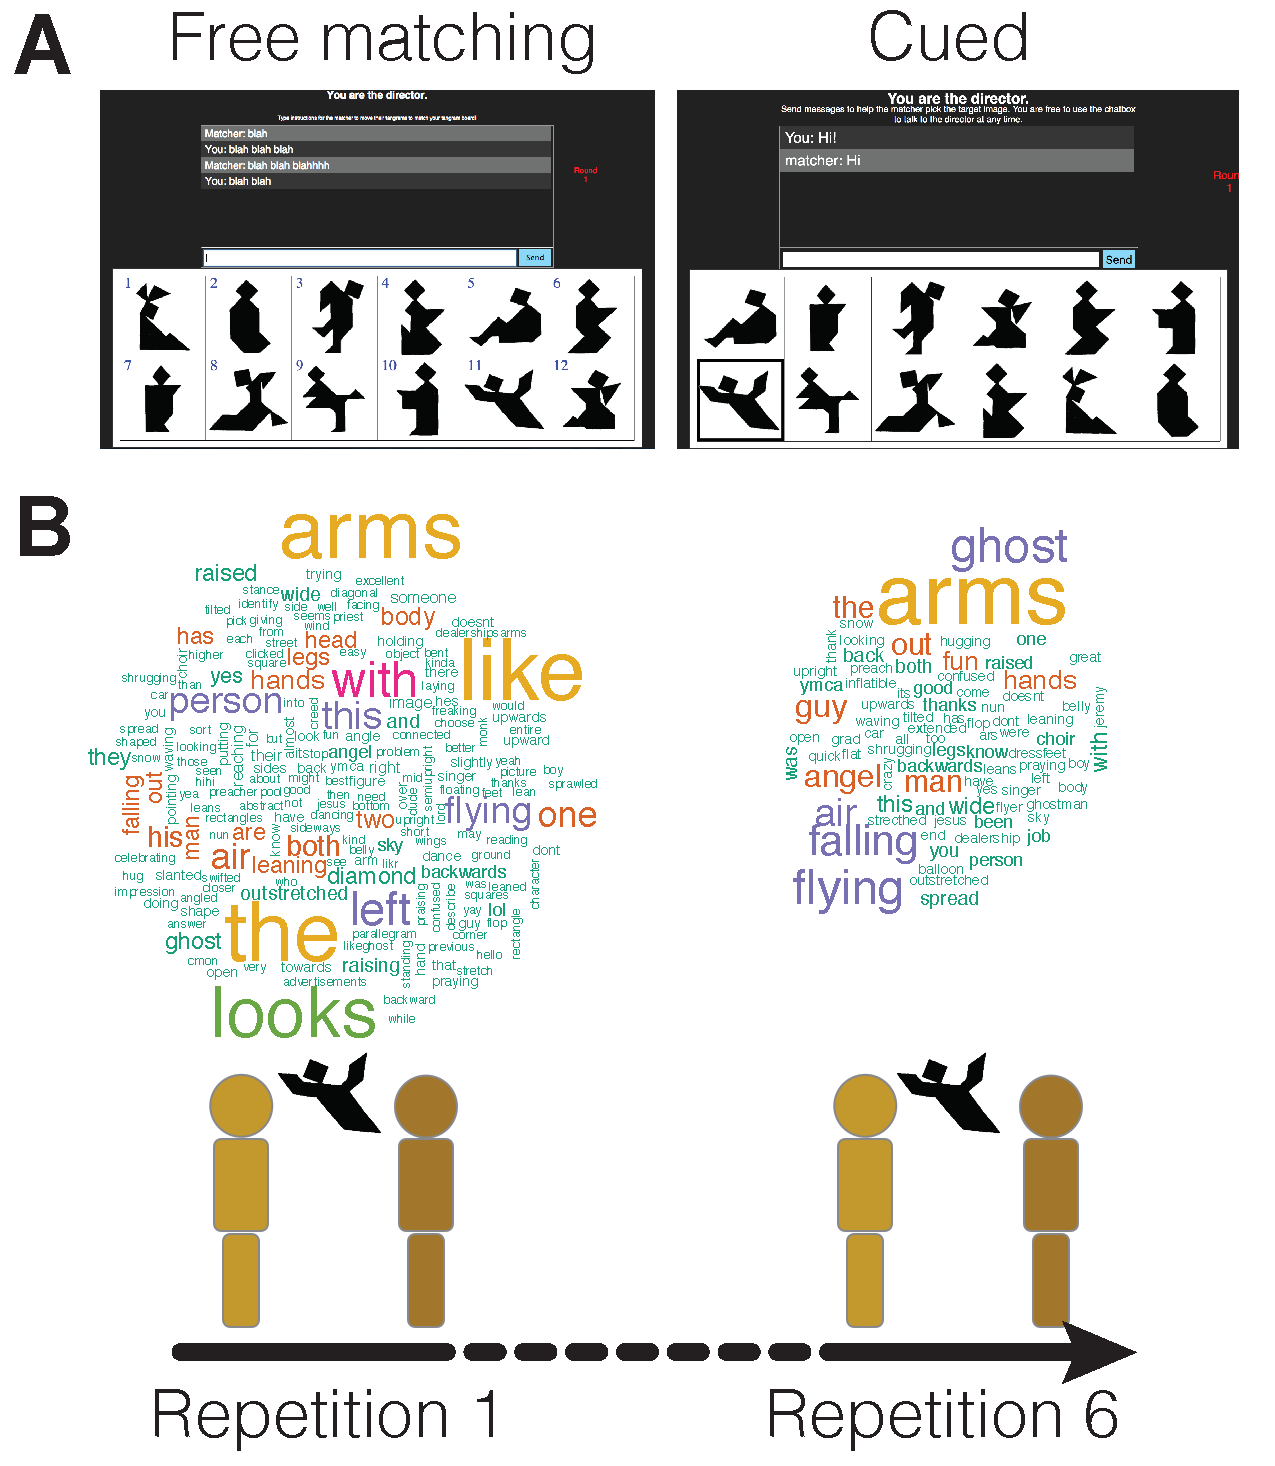
\includegraphics[scale=.9]{designAndExample.pdf}
\caption{`Free matching' and `cued' variants of the tangrams task.}
\label{fig:design}
\end{figure}

To collect a large corpus of natural dialogue that allows us to measure how pairs coordinate on meaning over time, we faced two primary decisions.
First, to observe the formative period of linguistic conventions, we required novel, ambiguous stimuli for which participants didn't already have strong initial conventions.
Second, to observe the \emph{dynamics} of conventions over time, we needed the same coordination problem to be repeated over time, such that earlier outcomes are relevant for later decisions.
These criteria are satisfied by a \emph{repeated reference game} design in which participants refer to the same objects across multiple rounds as they build up a shared history of interaction, or common ground, with their partner. 

We developed two variants of the game: a relatively unconstrained \emph{free-matching} version that more closely replicates the classic in-lab design, and a more tightly controlled \emph{cued} version that allows for higher resolution analyses of how references to individual tangrams changed over time (see Fig. \ref{fig:design}). 
The \emph{free-matching} version was an exploratory sample, but we pre-registered our full pre-processing and analysis pipeline for the \emph{cued} version\footnote{osf.io/XXXXX}. While we report results for both versions throughout, we privilege the \emph{cued} version as our confirmatory sample.

\subsubsection{Participants}\label{participants}

A total of 480 participants (218 in the \emph{free-matching} version and 262 in the \emph{cued} version) were recruited from Amazon's Mechanical Turk and paired into dyads to play a real-time communication game using the framework in \cite{Hawkins15_RealTimeWebExperiments}. 

\subsubsection{Exclusion criteria}

After excluding games that terminated before the completion of the experiment due to server error or network disconnection (40 in \emph{free matching} and 33 in \emph{cued}), as well as games where participants reported a native language different from English (2 in \emph{free matching} and 3 in \emph{cued}), we implemented an additional exclusion criterion based on accuracy. 
% Because the classic work using the repeated reference game paradigm reported near ceiling accuracy for all pairs, and b
We used a 66/66 rule, excluding pairs that got fewer than 66\% of the tangrams correct ($\ge8$ of 12) on more than 66\% of blocks ($\ge4$ of 6). 
While the most pairs were near ceiling accuracy by the final round, this rule excluded 11 in \emph{free matching} and 8 in \emph{cued} who appeared to be guessing or rushing to completion. 
After all exclusions, we were left with a \emph{free matching} corpus containing a total of 8,639 messages over 56 complete games and a \emph{cued} corpus containing 9,164 messages over 83 games.

\subsubsection{Stimuli \& Procedure}\label{stimuli}

On every trial, participants were shown a \(6 \times 2\) grid containing twelve tangram shapes, reproduced from \cite{ClarkWilkesGibbs86_ReferringCollaborative}.  
After passing a short quiz about task instructions, participants were randomly assigned the role of either `director' or `matcher' and automatically paired into virtual rooms containing a chat box and the grid of stimuli. 
Both participants could freely use the chat box to communicate at any time. 

In the \emph{free-matching} version, our procedure closely followed \cite{ClarkWilkesGibbs86_ReferringCollaborative}. 
The director and matcher began each round with scrambled boards. 
The director's tangrams were fixed in place, but the matcher's could be clicked and dragged into new positions.
The players was instructed to communicate through the chat box such that the matcher could rearrange their shapes to match the order of the director's board.
When the players were satisfied that their boards matched, the matcher clicked a `submit' button that gave players batched feedback on their score (out of 12) and scrambled the tangrams for the next round. 
After six rounds, players were redirected to a short exit survey. 
Cells were labeled with fixed numbers from one to twelve in order to help participants easily refer to locations in the grid (see Fig. \ref{fig:design}).

While this replicated design allows for highly naturalistic interaction, it poses several problems for text-based analyses. 
First, utterances must contain not only descriptions of the tangrams but also information about the intended location (e.g. '\emph{number 10} is the \dots'). 
Additionally, because there were no constraints on the sequence, participants can revisit tangrams out of order or mention multiple tangrams in a single message, making it difficult to isolate exactly which utterances referred to which tangrams without extensive hand-annotation. 
Finally, the design of the `submit' button made it easy for players to occasionally advance to the next round without referring to all 12 tangrams. 

For the \emph{cued} version, then, we designed a more straightforwardly sequential variation on the task where speakers are privately cued to refer to targets one-by-one and feedback is given on each round (see Fig. \ref{fig:design}); this allows us to straightforwardly conduct analyses at the tangram-by-tangram level. 
On each trial, one of the twelve tangrams was privately highlighted for the director as the \emph{target}. 
Instead of clicking and dragging into place, matchers simply clicked the one they believed was the target. 
They were not allowed to click until after a message was sent by the speaker.  
We constructed a sequence of six blocks of twelve trials (for a total of 72 trials), where each tangram appeared once per block.
Because targets were cued one at a time, numbers labeling each square in the grid were irrelevant and we removed them. 
The context of tangrams was scrambled on every trial, and participants were given full, immediate feedback: the director saw which tangram their partner clicked, and the matcher saw the intended tangram.

\subsubsection{Data pre-processing}

We used a three step pre-processing pipeline to prepare our corpus for subsequent analyses. Unless otherwise noted, we used the open-source Python package \texttt{spaCy} to implement all NLP tasks. 

\begin{enumerate}

\item \textbf{Spell-checking and regularization}: We conservatively extracted all tokens that did not exist in the vocabulary of the smallest available ($\sim$ 50,000 word) \texttt{spaCy} model and passed them through the SymSpell spell-checker \footnote{\texttt{https://github.com/wolfgarbe/SymSpell}}. These suggested corrections were then sequentially presented to the first author and either accepted or overridden at their judgement. This process constructed a reproducible spell-correction dictionary we applied to our dataset.

\item \textbf{Cleaning unrelated discourse}: Because we allowed our participants to interact in real-time through the chat box, many pairs produced text unrelated to the task of referring to the current target (e.g. greeting one another, asking personal questions, commenting on the length of the task or the results of previous rounds). We wanted to ensure that our structural results were not confounded by patterns in this kind of discourse across the task, and that the semantic content we observe on a particular trial is in fact being used to refer to the current target rather than task-irrelevant topics or, as we found in some cases, referring to other tangrams while debriefing previous errors. We therefore applied a manual pass applying a rubric that any text not directly referring to the current target is removed. For example, utterances like ``this is the one we got wrong last time'' were kept in because they were referring to a property of the current tangram, but utterances like ``good job'' and ``they'll go quicker if you remember what I say!'' are not. This process also created a reproducible JSON.

\item \textbf{Collapsing multiple messages within a round}: Finally, some speakers used our chat box like an texting interface, hitting the enter key between every micro-phrase of text. This made it difficult to interpret the output of syntactic parses. We therefore collapsed repeated messages by a participant within a round into a single message by inserting commas between successive messages. We chose to use commas because it tends to maintain grammaticality and does not inflate word counts.

\end{enumerate}

%Still, we verified that all results reported were robust to these exclusion criteria, and to our data pre-processing steps\todo{check}.

\section{Results: characterizing the dynamics of content}

The inferential account laid out in earlier chapters makes three key predictions about how speakers change the content of their referring expressions over time.
\emph{First}, if participants are influenced by pragmatic pressures to be informative, the labels that conventionalize should not be a random draw from the initial description. 
Instead, we predict that more \emph{distinctive} words in initially successful labels (e.g. words used exclusively to describe one tangram) will be more likely to remain in later descriptions.
\emph{Second}, due to sources of variability in the population of speakers, we predict that the referring expressions used by different pairs will increasingly diverge to different, idiosyncratic labels.
In other words, different pairs will find different but equally successful equilibria in the space of possible linguistic conventions.
\emph{Third}, as speakers learn and gradually strengthen their expectations about how their partner will interpret their referring expressions, the labels used within each pair for each tangram with stabilize.
In other words, once there is evidence that a particular label is successfully understood, there is little reason to deviate from it.

\subsection{Initially distinctive words are more likely to conventionalize}
\label{sec:distinctive}

We begin by investigating \emph{which} content is dropped and which is preserved.
Which computational principles may allow us to predict whether a particular word in a speaker's initial description of an object will become established as a convention for referring to it on later rounds?
In previous chapters, we discussed two principles that are particular relevant for this question.
First, if speakers are attempting to be informative \emph{in this particular context of tangrams} then the Gricean maxim of quality suggests that a good referring expression is one that applies more strongly to the target than to the distractors. 
Properties that are shared in common across multiple objects are poor candidates for conventions that must distinguish among them.
Second, the principles of cross-situational meaning adaptation suggest that these informativity considerations will be strengthened through learning.
The exclusive usage of a word with one tangram and no others should reinforce the specificity of that meaning in the local discourse context, even if the listener may be \emph{a priori} willing to extend it to other targets.
Conversely, if a particular word has been successfully used with several different referents, its specificity may be weakened in the local context.
Putting these principles together, we hypothesized that more \emph{initially distinctive} words would be more likely to conventionalize.


For each pair of participants, we quantified the distinctiveness of a word $w$ as $n_w$: the number of tangrams that it was used to describe on the first repetition. 
A word that is only used in the description of a single tangram (e.g. a descriptive noun like ``rabbit'') would be very distinctive, while a word used with all 12 tangrams (e.g. an article like ``the'') would be not distinctive at all.
While this formulation is the most transparent to state in words, it is equivalent (up to a constant) to two popular  and theoretically motivated measures of distinctiveness used in natural language processing \cite{salton1988term}.
The first is \emph{term frequency-inverse document frequency} \cite<tf-idf;>{sparck1972statistical}, which multiplies the term frequency $tf(w,d)$ of a word $w$ in a document $d$ by a ``global'' term $\log(N/n_w)$ where $N$ is the total number of documents and $n_w$ is the number of documents containing $w$. 
In our case, the ``documents'' are just the referring expressions used for a distinct tangram on the first round, so $N=12$ and we can take $tf(w,d)$ to be a boolean for simplicity: 1 if the word occurs, 0 if it does not.
We can thus retrieve our simpler measure by exponentiating, dividing by $12$, and taking the inverse.
The second is \emph{positive point-wise mutual information} (PPMI). 
Point-wise mutual information compares the joint probability of a word occurring with a particular tangram to the probability of the two occurring independently: 
$$PMI_{word, tangram} = \log\frac{P(word, tangram)}{P(word)P(tangram)}$$
\emph{Positive} point-wise mutual information is given by $\min(0, PMI)$, restricting the lower bound to 0. 
It can be shown for our case that \emph{tf-idf} is the maximum likelihood estimator for PPMI: the numerator reduces to a boolean when we only have one observation per tangram \cite{robertson2004understanding}.

\begin{figure}[t!]
\centering
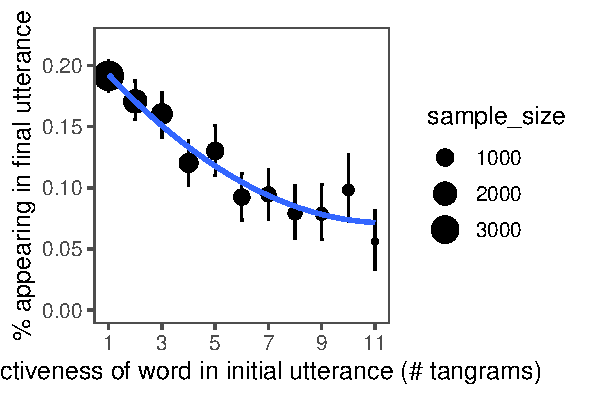
\includegraphics[scale=.9]{distinctiveness.pdf}
\caption{Error bars are bootstrapped 95\% CIs.}
\label{fig:distinct}
\end{figure}

Given this measure of word distinctiveness at the speaker-by-speaker level, we were interested in the extent to which it accounts for \emph{conventionalization}, the probability that a word in the speaker's initial description is preserved until the end of the game. 
More than half of the words used to refer to a tangram on the final round (57\%) appeared in the initial utterance. \footnote{The 43\% of final round words that did not exactly match were often synonyms or otherwise semantically related to words used on the first round, e.g. ``foot'' on the first round and ``leg'' on the last. In other cases, the labels used at the end were introduced after the first repetition, e.g. one pair only started using the label ``portrait'' on repetition 3.}
We thus restricted our attention to this subset of words, coding them with a 1 if they later appeared in the final round and 0 if they did not.
We then ran a mixed-effects logistic regression including a fixed effect of initial `distinctiveness (\emph{tf-idf}) and maximal random effect structure with intercepts and slopes for each tangram and pair of participants.
We found a significant positive effect of distinctiveness: words that were used with fewer tangrams on the initial round were more likely to conventionalize, $b = 0.42, z = 5.4$ (see Fig. \ref{fig:distinct}).

\subsection{Conventions diverge across pairs and stabilize within pairs}

To jointly examine our other predictions about the dynamics of content, we introduce two different quantitative measures of similarity: one based on distances computed between continuous vector embeddings of referring expressions and the other based on properties of the discrete word count distribution.
Because these analyses depend on tangram-level resolution, we only examine the ``cued'' dataset in this section.

\paragraph{Measuring convergence and divergence with discrete word distributions}

examine the discrete \emph{distribution of words} that each pair uses to refer to each tangram.
If a pair of participants converges on stable labels for a tangram, then this stability should manifest in a highly structured distribution over words throughout the game for that pair.
If different speakers discover diverging conventions, this idiosyncracy should also manifest in differing word distributions.
We formalize these intuitions by examining the information-theoretic measure of entropy: $$H(W) = \sum_w P(w) \log P(w)$$
The entropy of the word distribution for a pair is maximized when all words are used equally often and declines as the distribution becomes more structured, i.e.~when the probability mass is more concentrated on a subset of words.

To compare word distributions across games, we use a permutation test methodology.
By scrambling utterances across games and recomputing the entropy of the scrambled word distribution, we effectively disrupt any distinctive structure within each pair.
There are two important inferences we can draw from this test.
First, in a null scenario where different pairs did \emph{not} diverge as predicted and instead every pair coordinated on roughly the same (optimal) convention for each tangram, this permutation operation would have no effect since it would be mixing together 
Second, in another null scenario where pairs did not converge and instead varied wildly in the words they used on each round, permuting across games would also have no effect since it would simply mix together word distributions that already have high entropy.
Hence, scrambling should \emph{increase} the average game's entropy only in the case where both predictions hold: each game's idiosyncratic, concentrated distribution of words would be mixed together to form more heterogeneous and therefore high-entropy distributions.

Following this logic, we computed the average within-game entropy for 1000 different permutations of speaker utterances. 
We permuted utterances within rounds rather than across the entire data set to control for the fact that earlier rounds may generically differ from later rounds. 
Since this permutation scheme keeps the number of messages per participant constant and simply swaps out the content of those messages, it also controls for the fact that some speakers sent more messages than others. 
We found that our null distribution lay within the interval $X, Y$, which is significantly higher than the true entropy (averaged across games) of $Z, p < 0.001$.

\paragraph{Measuring similarity using vector space embeddings} 
An alternative way to quantify convergence within and divergence across different pairs is to use a continuous similarity between vector space embeddings of utterances.
Although the idea of using dense vector space representations of words to measure similarity is an old one \cite{osgood1952nature,landauer_solution_1997,bengio_neural_2003}, recent breakthroughs in machine learning have yielded rapid improvements in these representations \cite<e.g>{mikolov2013distributed,pennington2014glove}.
To quantify the dynamics of semantic context in referring expressions across and within games, we extracted the 300-dimensional GloVe vector for each word. 
We then averaged these word vectors to obtain a single sentence vector for each referring expression\footnote{Variations on such naive averaging methods are surprisingly strong baselines for sentence representations \cite{arora2017asimple}, performing better than supervised LSTM representations or unsupervised skip-thought vectors \cite{KirosEtAl15_SkipThought}}.
To avoid artifacts from function words, we only included open-class content words (nouns, adjectives, verbs) in this average.
We can then define a similarity metric between any pair of vectors $\langle u_i, u_j \rangle$.
We find that our results are robust to several choices of metric, but for simplicity we will use cosine similarity $$\cos \theta_{ij} = \frac{u_i \cdot u_j}{\| u_i\| \| u_j \|}$$ throughout the presentation below.

\begin{figure}[t!]
\centering
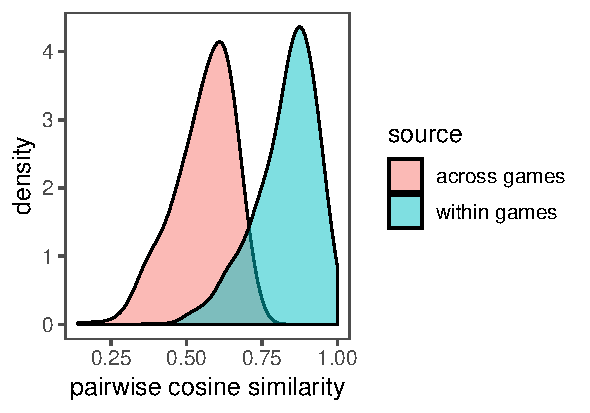
\includegraphics[scale=.9]{across_vs_within.pdf}
\caption{Distribution of similarities between different utterances within and across different games.}
\label{fig:withinvsacross}
\end{figure}

\paragraph{Utterances are more similar overall within games than between games}  
Before examining the dynamics of these vectors, we first test the basic prediction that utterances \emph{within} a game are more similar overall than utterances \emph{across} games, reflecting systematic variability in how different pairs solve the referential challenge posed by the reference game.
For each tangram, we computed the pairwise similarity between all utterances \emph{within} a game and also \emph{across} games. 
The distributions of these values are shown in Fig. \ref{fig:withinvsacross}.
We estimated the distance between these distributions using the standard normalized sensitivity $d' = \frac{\mu_A - \mu_W}{\sqrt{1/2(\sigma^2_A+\sigma^2_W)}} = 2.71$.
To compare this estimated difference against the null hypotheses that within- and across-game similarities are drawn from the same distribution, we conducted a permutation test by scrambling `within' and `across' labels for each similarity and re-computing $d'$ 1000 times. 
We found that our observed value was extremely unlikely under this null distribution, $95\%~CI: [-0.09, 0.09], p < 0.001$. 

In other words, utterances from a single pair tend to cluster together in semantic space while different pairs are more spread out in different parts of the space.
This observation is consistent with our hypothesis that different pairs discover different conventions while a single pair tends to keep using a convention once established.
Having established this separation between similarity distributions in aggregate, we proceed to ask more fine-grained questions about the \emph{dynamics} through space: how do individual pairs evolve in their content over successive rounds?
To more rigorously test our predictions about gradual divergence to multiple equilibria and convergence to internally stable conventions, we conducted three analyses directly on the semantic vectors.

\paragraph{Increasing dissimilarity from initial utterance}

First, we hypothesized that there was cumulative change in the semantic content of a particular pair's utterances across repetitions.
Concretely, we predicted that within a particular pair of participants, utterances on later repetitions would become increasingly dissimilar from the initial utterance.
We tested this prediction in a mixed-effects regression model including (orthogonalized) linear and quadratic fixed effects of the `lag' from the first repetition (i.e. 1 for the second repetition, 2 for the third repetition, etc) as well as maximal random effects for each tangram and pair of participants.
We found a significant linear decrease in similarity to the initial round as the lag becomes larger, $b = -3.5,~t = 12.2$, as well as a significant quadratic term, $b=1.1, t=5.3$, suggesting that this decrease in similarity slows down over time (see Fig.~\ref{within-across}A).

However, since the entire distribution of utterances may have drifted to a different region of the semantic space for generic reasons (e.g., because they were shorter overall), we compared the estimated drift \emph{within} pairs of participants to a permuted baseline.
For each target tangram, we scrambled utterances across different pairs of participants and re-ran our mixed-effects model to obtain a null distribution representing the decrease in semantic distance from a \emph{random} speaker's utterance on the first round.
We found that this permuted baseline also showed a linear decrease over time, but our true estimate ($b=-3.5$) fell narrowly outside the null distribution of effects $(95\%~CI= [-3.34, -3.04])$, showing that utterances by a particular speaker drifted from their own initial utterance to a slightly greater degree than would be expected due to generic differences between utterances made at different timepoints in an interaction \footnote{Both here and for the permuted baselines in the subsequent two analyses we needed to simplify the random effects structure to contain only random intercepts due to convergence issues over the large number of permutations. However, we were interested in the coefficient estimate rather than statistical significance in these permuted models, and estimates appeared stable across different random effects structures.}.
This difference is likely a consequence of random utterances from different speakers being more dissimilar even on \emph{early} repetitions, thus depressing the overall slope.
%We expect that this is a consequence of random pairs beginning as  the beginning, depressing 

\begin{figure}
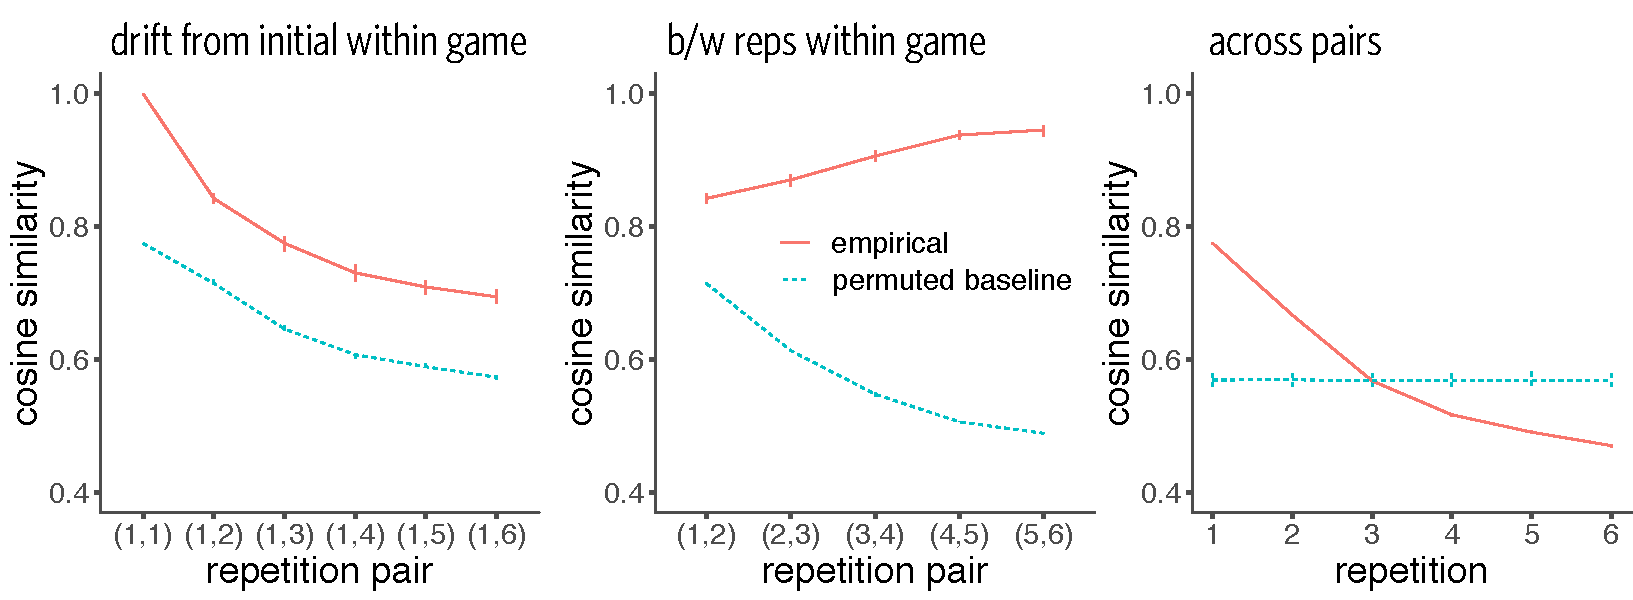
\includegraphics[scale=.5]{similarity_analysis.pdf}
\caption{Utterances within a pair (A) become more dissimilar from initial utterance and (B) become more similar to successive utterances on later repetitions, but (C) utterances across pairs become steadily more dissimilar.}
\label{fig:similarity}
\end{figure}

\paragraph{Increasing internal consistency within interaction}

As speakers modified their utterances across successive repetitions, we additionally hypothesized that they would converge on increasingly consistent ways of referring to each tangram.
To test this prediction, we computed the semantic similarity between successive utterances produced by each speaker when referring to same tangram (i.e.~repetition $k$ to $k+1$). %.^, and evaluated how this similarity changed across repetitions.
A mixed-effects model with linear and quadratic fixed effects of repetition number and maximal random effects for both tangram and pair of participants showed that similarity between successive utterances increased substantially throughout an interaction ($b = 2.7,~t = 10.9$; Fig.~\ref{within-across}B). 
The quadratic term was not significant ($b= -0.4,~t=-1.8$).
Again, we compared our empirical estimate of the magnitude of this trend to a null distribution of slopes estimated by scrambling utterances across pairs and re-running the regression model.% to disrupt the consistency of interactions.
The estimated slope fell outside this null distribution, for which similarity was strongly \emph{decreasing}, $CI = [-5.9, -5.4]$, providing evidence that increasingly consistent ways of referring to each object manifested only for series of utterances produced within the same interaction.

\paragraph{Increasingly different content across interactions}
Finally, we predicted that the way different pairs refer to the same tangram would become increasingly dissimilar from each other across repetitions, gradually diverging into different equilibria.
We tested this prediction by computing the mean pairwise similarity between utterances used by different speakers to refer to the same object.
The large sample of pairwise similarities ($N = 257,040 = 12~\textrm{tangrams} \times 6~\textrm{repetitions} \times \frac{85 \cdot 84}{2}~\textrm{distinct pairs}$) presented both advantages and disadvantages.
On one hand, we could obtain highly reliable estimates of mean similarity. 
On the other hand, larger random-effects structures led to convergence problems.
We therefore ran a mixed-effects regression model including linear and quadratic fixed effects of repetition number including maximal random effects only at the tangram-level. 
We found a strong negative linear fixed effect of repetition on between-game semantic similarity ($b = -50.7, t= 16.8$) as well as a significant quadratic effect ($b= 16.1, t = 12$), indicating that this divergence slows over time as each pair stabilizes, (see Fig.~\ref{within-across}C).
We again conducted a permutation test to compare this $t$ value with what would be expected from scrambling utterances across repetitions for each pair and target.
We found that the estimated slope was highly unlikely under this distribution $(CI = -2.5, 2.9],~p~<~0.001)$. 


\begin{figure}[t!]
\centering
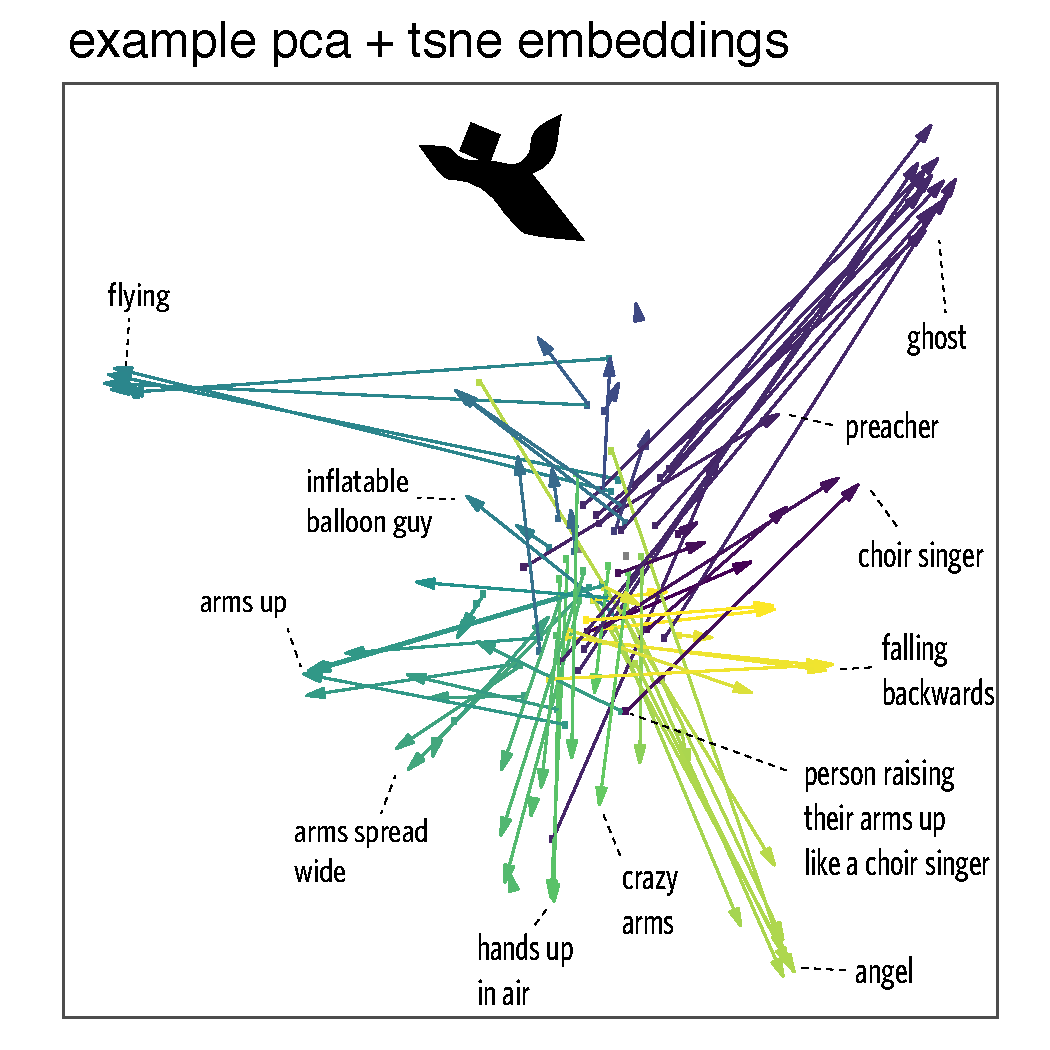
\includegraphics[scale=.6]{tsne-tangramC_annotated.pdf}
\caption{2D projection of semantic embeddings for example tangram. Each arrow represents the trajectory between the first round to last round for a distinct pair of participants. Color represents the rotational angle of the final location to more easily see where each pair began. Annotations are provided for select utterances, representing different equilibria found by different participants.}
\label{fig:tsne}
\end{figure}


\paragraph{Visualizing trajectories through vector space}  
Finally, to better understand the changes uncovered by these analyses of utterance embeddings, we visualize the trajectories taken by each pair of participants when referring to a particular example tangram, annotating utterances in several parts of the space.
First, we took the first 50 components recovered by running Principal Components Analysis (PCA) on the 300-dimensional utterance embeddings. 
We then use t-SNE \cite{maaten2008visualizing} to stochastically embed the lower-dimensional PCA representation of each utterance in a common 2D vector space. 
In Fig. \ref{fig:tsne}, each arrow connects the first and last utterance a particular pair used to refer to this tangram.

We observe that the initial utterances of each game tend to cluster tightly near the center of the space and the final utterances are \emph{dispersed} more widely around the edges. 
This pattern is consistent with the hypothesis that different speakers overlap more in the content of their early descriptions before diverging to more distinctive different equilibria later in the game  (see \ref{sec:distinctive}). 
For this particular tangram, there were a handful of semantically distinct labels that served as equilibria for multiple pairs (``ghost,'' ``flying,'' ``angel'') as well as many more idiosyncratic labels.
Pairs often initially mentioned multiple properties (e.g. ``person raising their arms up like a choir singer'') before breaking the symmetry and collapsing to one of these properties (``choir singer'').
%Second, single pairs generally do not jump widely around the space; most trajectories are `spoke'-like, emitting from the center to near the end-state.
%This suggests that speakers converge fairly monotonically and consistently to their final utterances. 

\subsubsection{Discussion}

This discrete measure has both advantages and disadvantages compared to the continuous vector space measures above.
A key advantage is that the entropy is not dependent on any particular choice of pre-trained vector embedding. 
Due to biases in the training corpora, these representations may not capture some of the more idiosyncratic conventions that participants converge on (e.g. ``YMCA'' or ``zig zag'' or ``Frank'' -- short for ``Frankenstein'').
To the extent we find converging results, the discrete measure may address concerns about the quality of the continuous representation.
A disadvantage is that the entropy is sensitive to the support of the word distribution --- the vocabulary present in the corpus on a particular round --- and thus does not have a natural scale.
Additionally, because it is based entirely on the frequency of tokens, it may treat even close synonyms as entirely distinct tokens in the word distribution. 

\section{Results: characterizing the dynamics of structure}\label{results}

Having established \dots

\subsection{Dialogue between speaker and listener}\label{listener-feedback}

Before focusing our analysis on the rich dynamics of how \emph{directors} produce referring expressions over time, we first examine the bi-directional dynamics of dialogue exchanges. 
An influential result from is that conceptual pacts for referring are established \emph{collaboratively} \cite[see also \cite{KraussWeinheimer66_Tangrams, GarrodFayLeeOberlanderMacLeod07_GraphicalSymbolSystems}]{ClarkWilkesGibbs86_ReferringCollaborative}: 
directors and matchers engage in a bi-directional process where matchers ask follow-up questions, suggest corrections, and acknowledge or verbally confirm their understanding through a backchannel. 
This theory predicts that (1) listener feedback should be highest on the first round and drop off once meanings are agreed upon, and (2) dyads with more initial listener feedback should reduce to more efficient conventions. 
Our use of a chat box rather than in-person verbal communication, along with the automatic feedback we provided each round in the \emph{cued} condition, may have diminished the bi-directionality somewhat, but we find correlational evidence of both patterns in our uncollapsed but otherwise cleaned data. 
The number of listener messages decreases significantly over the game $(b=-0.5, t = -10.6, p < 0.001)$, and there is a small but significant effect of the (logged) number of initial listener messages on overall \% reduction in the number of words used by the director, $r = 0.26, 95\% CI = [0.57, 0.45], p = 0.014$.
\todo[inline]{Note: this last result isn't actually saying much because when listeners say more on the first round, speaker often say more in response\dots they therefore have a higher initial word count to reduce from than if the listener didn't say anything, so it's not surprising that \% reduction is larger... we need to revise the analysis to control for this, e.g. by only considering reduction from the words used \emph{before} the listener's first message, i.e. what they \emph{would} have initially said if the listener didn't chime in? The more simple \& obvious regression formulation would be whether \# of initial listener messages predicts \emph{absolute} round 6 message length rather than \% reduction; this didn't come out, but I switched to the \% reduction version because I was worried that it was just due to pair-level variance in final round length}
\todo[inline]{This could also be a good place to put an effect of, like, more words used for tangrams that were incorrect in the previous round.}

\begin{figure}[t]
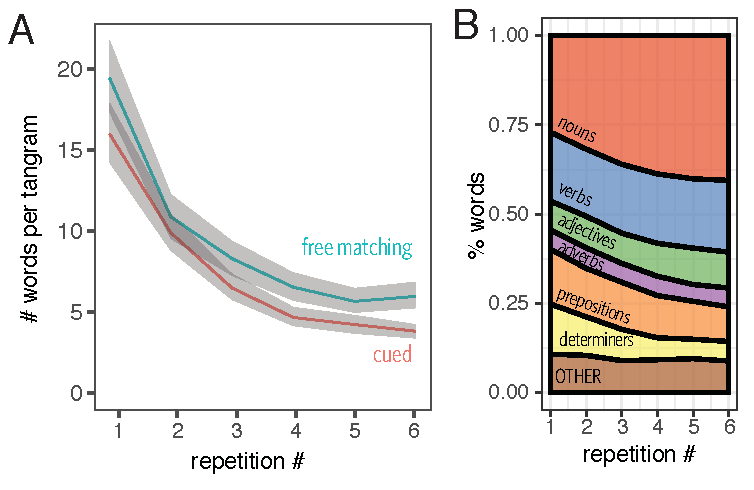
\includegraphics[scale=.65]{reduction.pdf}
\caption{(A) similar reduction in \# words per tangram for both variants of the task (B) word counts broken down by part of speech, combined across both variants (C) phrasal reduction based on syntactic parse \todo[inline]{Maybe showing \% reduction is better than raw numbers, i.e. normalizing by occurrence on first round (or version mike suggested w/ bars showing proportions at beginning and end.}}
\label{fig:reduction}
\end{figure}

\subsection{Reduction in number of words}\label{reduction}

Next, we turn to a set of analyses examining reduction in utterance length over the course of the experiment. 
At the coarsest level, we find that the mean number of words used by speakers decreases over time (see Fig. \ref{fig:replication}). 
This decrease replicates a highly reliable reduction effect found throughout the literature on iterated reference games (Brennan \& Clark, 1996; Krauss \& Weinheimer, 1964), although perhaps due to our purely textual (vs.~spoken) interface, participants in our task used many fewer words overall than previously reported. 
The following analyses break down this broad reduction into a finer-grained set of phenomena.

\subsection{Reduction in parts of speech}
The next level of granularity motivating our model approach concerns which kinds of words are most likely to be dropped. 
Is the speaker adopting a shorthand where they drop uninformative function words, or are they simplifying or narrowing their descriptions by omitting meaningful details (Clark \& Wilkes-Gibbs, 1986)? 
We used the Stanford CoreNLP part-of-speech tagger (Toutanova, Klein, Manning, \& Singer, 2003) to count the number of words belonging to each part of speech in each message. Fig. \ref{fig:pos} shows the percent reduction of different parts of speech from the first round to the sixth round. 
We find that determiners (`the', `a', `an') are the most likely class of words to be dropped with an X\% reduction rate, on average. 
Nouns (`dancer', `rabbit') are the least likely class to be dropped with only an Y\% rate. 
Closed-class parts of speech are strictly more likely to be dropped than open-class parts of speech.

While this finding suggests that speakers might just be adopting a
shorthand using more ungrammatical fragments as the game proceeds, we
find a more complex dynamic by examining the table of unigrams and
bigrams most likely to be dropped (see Table \ref{tab:words}). Note that
alongside dropped articles, there are a number of words that form
conjunctions (`and') and modifiers (`of', `with', `the right'). In other
words, it may be more likely that when function words are dropped, it is
primarily as part of larger grammatical units that provide additional
information in identifying the target.

\subsection{Reduction in syntactic constituents}
We explicitly examined this hypothesis by running the Stanford
constituency parser (Schuster \& Manning, 2016), tagging the occurrence
of subordinate/adverbial clauses (`sitting \emph{facing left}') and
adjectival clauses (`angel \emph{that is praying}').\footnote{Specifically,
  we used the Universal Dependencies tags \texttt{csubj, ccomp, xcomp},
  and \texttt{advcl} for subordinate clauses and \texttt{acl} for
  adjectival clauses (Schuster \& Manning, 2016)} We found that both
were reduced over the course of the game (see Fig.
\ref{fig:replication}), lending additional support for the hypothesis
that meaningful details are increasingly omitted. Initial phrases pile
on multiple ambiguous, partially redundant modifiers and descriptors: as
the game progresses and ambiguity of reference decreases, these
additional meaningful units become less useful and can be dropped.

This result accords with early observations by \cite{Carroll80_NamingHedges}, which found that in three-quarters of transcripts from \cite{KraussWeinheimer64_ReferencePhrases} the short names that participants converged upon were prominent in some syntactic construction at the beginning, often as a head noun that was initially modified or qualified by other information. 

\subsection{Shared dynamics across pairs}

Tree-edit distance\dots


\section{Discussion}\label{general-discussion}

In this paper, we revisited the classic phenomenon of
convention-formation in a large-scale replication of the tangrams task,
finding evidence of arbitrariness and stability as well as finer-grained
reduction of meaningful clauses. 

%% Paragraph about opportunities for computational models
While we have focused on broader theoretical questions, our results also serve as a foundation for high-resolution task-performing computational models of communication seeking to explain the full richness of natural data. To build machines that naturally adapt to their interlocutors in human-robot or human-computer interaction scenarios, we must go behind qualitative efforts.

Theories of convention-formation vary in the extent to which social
reasoning about common ground is required. Our agents lie on a spectrum
between the heuristic updating agents of Barr (2004) and the
sophisticated agents of Clark \& Wilkes-Gibbs (1986), who
collaboratively build up explicit representations of mutual knowledge.
Speakers and listeners in our model implicitly coordinate their beliefs
through a shared history of observations, which serves as ``common
ground'' in an informal sense. They make critical use of pragmatic,
social reasoning in order to learn meanings, but do not explicitly
consider the fact that this history is shared, or represent their
partner's own uncertainty.

By capturing reduction, which purely heuristic theories have not yet
demonstrated, we showed that minimal assumptions of social reasoning go
a long way in accounting for key phenomena. Still, our model falls short
in some ways. For instance, because we do not provide a mechanisms for
the listener agent to respond with confirmation, repair, or follow-up
questions, we cannot make explicit predictions about the reduction in
\emph{listener messages} (as in Fig. \ref{fig:replication}) or the
impact of early listener responses on conventionalization. These
phenomena require our model to deal with planning over extended
dialogues, and to potentially weaken the assumption that one's partner
knows the true lexicon with complete certainty. Similarly, while our
model was explicitly designed with linguistic conventions in mind, it
remains to be seen whether the same formulation generalizes to broader
behavioral conventions. For example, the real-time coordination games
used in Hawkins \& Goldstone (2016) may not require players to reason
about a structured lexicon with noise, but an action policy
representation may play a similar role. While there remain many complex
aspects of convention-formation in communication games left for future
research, our approach nonetheless serves as a lower bound on the degree
of social reasoning needed to capture lexical conventions in these
games.